% The packages used here are just a sample. You may need others, and may not need some of these. It doesn't hurt to leave them in, unless they start to conflict with other packages you've added. Chapter 2 has example code for equations, figures, tables, citations, abbreviations, etc. If there are sections labeled 'optional' that you don't want, just comment them out. -jg

\documentclass[reqno,12pt,oneside]{report} % right-side equation numbering, 12 point font, print one-sided 
%\documentclass[reqno,12pt,twoside,openright]{report} % right-side equation numbering, 12 point font, print two-sided, Chapters start on odd pages. Rackham only accepts one-sided, so this is for personal printings.

\usepackage{rac}         % Use Rackham thesis style file
\usepackage{aas_macros}  % To allow the reading of ADS journal references in the bibliography
%\usepackage[intlimits]{amsmath} % Puts the limits of integrals on top and bottom
\usepackage{amsxtra}     % Use various AMS packages
\usepackage{amsthm}
\usepackage{amssymb}
\usepackage{amsfonts}
\usepackage{graphicx}    % Add some packages for figures. Read epslatex.pdf on ctan.tug.org
\usepackage{rotating}
\usepackage{color}
\usepackage{epsfig}
\usepackage{subfigure}   % To make subfigures. Read subfigure.pdf on ctan.tug.org
%\usepackage{caption}
%\usepackage{subcaption}
\usepackage{verbatim}
\usepackage{natbib}      % Allows you to use BibTeX
\usepackage[printonlyused]{acronym} % For the List of Abbreviations. Read acronym.pdf on ctan.tug.org
\usepackage{setspace}    % Allows you to specify the line spacing
%\doublespacing           % \onehalfspacing for 1.5 spacing, \doublespacing for 2.0 spacing.
\onehalfspacing
%\newcommand{\sun}{\ensuremath{\odot}} % sun symbol is \sun
%%%%%%%%%%%%%%%%%%%%%%%%%%%%%%%%%%%%%%%%%%%%%%%%%%%%%%%%%%%%%%%%%%%%%%%%%%%%%%%

% Various theorem environments. All of the following have the same numbering
% system as theorem.

\theoremstyle{plain}
\newtheorem{theorem}{Theorem}
\newtheorem{prop}[theorem]{Proposition}
\newtheorem{corollary}[theorem]{Corollary}
\newtheorem{lemma}[theorem]{Lemma}
\newtheorem{question}[theorem]{Question}
\newtheorem{conjecture}[theorem]{Conjecture}
\newtheorem{assumption}[theorem]{Assumption}

\theoremstyle{definition}
\newtheorem{definition}[theorem]{Definition}
\newtheorem{notation}[theorem]{Notation}
\newtheorem{condition}[theorem]{Condition}
\newtheorem{example}[theorem]{Example}
\newtheorem{introduction}[theorem]{Introduction}

\theoremstyle{remark}
\newtheorem{remark}[theorem]{Remark}
%%%%%%%%%%%%%%%%%%%%%%%%%%%%%%%%%%%%%%%%%%%%%%%%%%%%%%%%%%%%%%%%%%%%%%%%%%%%%%%

\numberwithin{theorem}{chapter}     % Numbers theorems "x.y" where x
                                    % is the section number, y is the
                                    % theorem number

%\renewcommand{\thetheorem}{\arabic{chapter}.\arabic{theorem}}

%\makeatletter                      % This sequence of commands will
%\let\c@equation\c@theorem          % incorporate equation numbering
%\makeatother                       % into the theorem numbering scheme

%\renewcommand{\theenumi}{(\roman{enumi})}

%%%%%%%%%%%%%%%%%%%%%%%%%%%%%%%%%%%%%%%%%%%%%%%%%%%%%%%%%%%%%%%%%%%%%%%%%%%%%%

% If printing two-sided, this makes sure that any blank page at the 
% end of a chapter will not have a page number. 
\makeatletter
\def\cleardoublepage{\clearpage\if@twoside \ifodd\c@page\else
\hbox{}
\thispagestyle{empty}
\newpage
\if@twocolumn\hbox{}\newpage\fi\fi\fi}
\makeatother 

%%%%%%%%%%%%%%%%%%%%%%%%%%%%%%%%%%%%%%%%%%%%%%%%%%%%%%%%%%%%%%%%%%%%%%%%%%%%%%

%This command creates a box marked ``To Do'' around text.
%To use type \todo{  insert text here  }.

\newcommand{\todo}[1]{\vspace{5 mm}\par \noindent
\marginpar{\textsc{To Do}}
\framebox{\begin{minipage}[c]{0.95 \textwidth}
\tt\begin{center} #1 \end{center}\end{minipage}}\vspace{5 mm}\par}

%%%%%%%%%%%%%%%%%%%%%%%%%%%%%%%%%%%%%%%%%%%%%%%%%%%%%%%%%%%%%%%%%%%%%%%%%%%%%%%
\begin{document}

\bibliographystyle{agu04}    % Set the bibliography style. agu04, plain, alpha, etc.

% Title page as required by Rackham dissertation guidelines
\titlepage{Thesis Proposal: Database and System Design for Emerging Storage Technologies}{Steven Pelley}{Doctor of Philosophy}
{Computer Science and Engineering}{2013}
{Assistant Professor Thomas F. Wenisch, Chair\\
 Professor Peter M. Chen\\
 Assistant Professor Michael J. Cafarella\\
 Assistant Professor Zhengya Zhang}

% Begin the front matter as required by Rackham dissertation guidelines
\initializefrontsections

% Optional Frontispiece
%\frontispiece{
\includegraphics[width=6in]{Intro/Happy} Find a cool picture to go here.}

% Optional, but recommended, Copyright page
%\copyrightpage{Steven Pelley}

% Page numbering. If you don't include a frontispiece or copyright page, you'll need to change this for two-sided printing.
\makeatletter
\if@twoside \setcounter{page}{4} \else \setcounter{page}{0} \fi
\makeatother
 
% Optional Dedication page
%\dedicationpage{For all the people}

% Optional Acknowledgements page
%\startacknowledgementspage
%Thanks to the people who made this dissertation possible, especially those who put together a nice \LaTeX\, template for me to use.
%\label{Acknowledgements}

% Optional Preface page
%\startprefacepage
%\input{Preface}
%\label{Preface}

% Table of contents, list of figures, etc.
\tableofcontents     % Required
\listoffigures       % Required if there is more than one figure
%\listoftables        % Required if there is more than one table
%\listofmaps          % Required if there is more than one map
%\listofappendices    % Required if there is more than one appendix
\listofabbreviations % Optional. Abbreviations should be stored in a file named abbr.tex

% Optional in-dissertation Abstract Page
\startabstractpage
{Database and System Design for Emerging Storage Technologies}{Steven Pelley}{Chair: Thomas F. Wenisch}
Emerging storage technologies offer an alternative to disk that is durable and allows faster data access.
Flash memory, made popular by mobile devices, provides block access with low latency random reads.
New nonvolatile memories (NVRAM) are expected in upcoming years, presenting DRAM-like performance alongside persistent storage.
Wheres both technologies accelerate data accesses due to increased raw speed, used merely as disk replacements they may fail to achieve their full potentials.
Flash's asymmetric read/write access (i.e., reads execute faster than writes) opens new opportunities to optimize Flash-specific access.
Similarly, NVRAM's low latency persistent accesses allow new designs for high performance failure-resistant applications.

This thesis addresses software and hardware system design for such storage technologies.
First, I investigate analytics query optimization for Flash, expecting Flash's fast random access to require new query planning.
While intuition suggests scan and join selection should shift between disk and Flash, I find that query plans chosen assuming disk are already near-optimal for Flash.
Second, I examine new opportunities for durable, recoverable transaction processing with NVRAM.
Existing disk-based recovery mechanisms impose large software overheads, yet updating data in-place requires frequent device synchronization that limits throughput.
I introduce a new design, \GroupCommit, to amortize synchronization delays over many transactions, increasing throughput at some cost to transaction latency.
Finally, I propose a new framework for persistent programming and memory systems to enable high performance recoverable data structures with NVRAM, extending memory consistency with persistent semantics to introduce \emph{memory persistency}.

\label{Abstract}

\startthechapters 
% The individual files for each of the chapters are put here.
% Save each chapter of your thesis to a seperate tex file
% and then use the \input command to include this file in your
% thesis.  For instance you can save a file to "intro.tex" and 
% then type \section{Introduction}

Data center power consumption continues to grow at an alarming pace; it is projected to reach 100 billion kWh at an annual cost of \$7.4 billion within two years \cite{EPA07}, with a world-wide carbon-emissions impact similar to that of the entire Czech Republic \cite{Mankoff08}. In light of this trend, computer systems researchers, application designers, power and cooling engineers, and governmental bodies have all launched research efforts to improve data center energy efficiency.  These myriad efforts span numerous aspects of data center design (server architecture \cite{Lefurgy03,Meisner09}, scheduling \cite{Moore06, Parolini08},  power delivery systems \cite{Fan07}, cooling infrastructure \cite{Patel02}, etc.).  However, with few exceptions, existing efforts focus narrowly on energy-efficiency of single subsystems, without considering global interactions or implications across data center subsystems. 

As sophisticated power management features proliferate, the dynamic range of data center power draw (as a function of utilization) is increasing, and interactions among power management strategies across subsystems grow more complex; subsystems can no longer be analyzed in isolation.   Even questions that appear simple on their face can become quite complicated.

Reasoning about total data center power is difficult because of the diversity and complexity of data center infrastructure.  Five distinct sub-systems (designed and marketed by different industry segments) account for most of a data center's power draw:  (1) servers and storage systems, (2) power conditioning equipment, (3) cooling and humidification systems, (4) networking equipment, and (5) lighting/physical security.  Numerous sources have reported power breakdowns \cite{EPA07,Meisner09}; Table~\ref{table::PowerDistribution} illustrates a typical breakdown today.   The first three subsystems dominate and their power draw can vary drastically with data center utilization. Cooling power further depends on ambient weather conditions around the data center facility. Even the distribution of load in each subsystem can affect power draws, as the interactions among sub-systems are non-linear
%(e.g., thermal hot spots disproportionately increase cooling requirements).

In this paper, our objective is to provide tools to the computer systems community to assess and reason about total data center power.  Our approach is two-fold, targeting both \emph{data center simulation} and \emph{abstract analytic modeling}.  First, we have collected a set of detailed power models (from academic sources, industrial white papers, and product data sheets) for each critical component of data center infrastructure, which describe power draw as a function of environmental and load parameters.  Each model describes the power characteristics of a single device (i.e., one server or computer room air handler (CRAH)) and, as such, is suitable for integration into a detailed data center simulator.  We describe how these models interact (i.e., how utilization, power, and heat flow among components) and outline the design of such a simulator. To our knowledge, we are the first to describe an integrated data center simulation infrastructure; its implementation is underway.

Although these detailed models enable data center simulation, they do not allow direct analytic reasoning about total data center power.  Individual components' power draw vary non-linearly with localized conditions (i.e., temperature at a CRAH inlet, utilization of an individual server), that require detailed simulation to assess precisely.  Hence, to enable back-of-the-envelope reasoning, we develop an \emph{abstract model} that replaces key steps of the data center simulation process with simple parametric models that enable analysis of average behavior.  In particular, we abstract away time-varying scheduling/load distribution across servers and detailed tracking of the thermodynamics of data center airflow.  Our abstract model provides insight into how data center sub-systems interact and allows quick comparison of energy-efficiency optimizations.

\begin{table}[t]
\begin{center}
\caption{ \textbf{Typical Data Center Power Breakdown.} }
\label{table::PowerDistribution}

\begin{tabularx}{\linewidth}{c c c c c}
    \toprule
    Servers & Cooling & Power Cond. & Network & Lighting \\
    \midrule
    56\% & 30\% & 8\% & 5\% & 1\% \\
    \bottomrule
  \end{tabularx}
\end{center}

\end{table}
. 

 \chapter{Introduction}
 \label{chap:Intro}
 For decades disk has been the primary technology for durable and large-capacity storage.
Although inexpensive and dense, disk provides high performance only for coarse-grained sequential access and suffers enormous slowdowns for random reads and writes.
Recently, several new technologies have emerged as popular or viable storage alternatives.
Flash memory, primarily used for mobile storage, has gained traction as a high-performance enterprise storage solution.
Nonvolatile Random Access Memories (NVRAM), such as phase change memory and spin-transfer torque RAM, have emerged as high performance storage alternatives \cite{BurrKurdi08}.

These technologies offer significant performance improvements over disk, while still providing durability with great storage capacity.
As drop-in replacements for disk, Flash and NVRAM greatly accelerate storage access.
However, the disk interface fails to leverage specific device characteristics.
Section~\ref{sec:Background:Storage} provides a background on these storage technologies and specifically how their performance differs from disk.

This dissertation investigates how several data-centric workloads interact with future storage technologies, the relevant software and algorithms, and in some instances computer hardware.
Specifically, I consider analytics (commonly Decision Support Systems -- DSS -- popular in ``Big Data") and On-Line Transaction Processing (OLTP).
Both workload classes have been optimized to surmount disk's constraints, yet storage devices often remain the performance bottleneck and dominant cost.
I match each workload to the emerging storage technology that suits it best and address specific opportunities or deficiencies in the software and hardware systems.

\section{Analytics}
\label{sec:Intro:Analytics}

Analytics relies on disk to provide enormous data capacity.
Typical analytics work-flow involves taking a snapshot of data from an online database and mining this data for complex, yet useful, patterns.
While applications do not rely on disk's durability for recovery (in fact, instances that fit in main memory have no need for disk), modern analytics data sets reach peta-byte scale \cite{Economist10}, and accessing such large data imposes the dominant bottleneck.
Such capacity is currently achieved only by dense disk and Flash memory.

Decades of research have provided modern analytics databases with tools to minimize storage accesses, particularly slow random accesses (e.g., disk-specific indexes, join algorithms to minimize page access and produce large sequential runs).
Whereas these optimizations are still effective for Flash, they fail to leverage Flash's ability to quickly read non-sequential data (many optimizations purposefully avoid random access patterns on disk).
As examples, I consider access paths (various scan types) and join algorithms.
An historic rule of thumb for scans is that an index should be used when less than 10\% of rows in a table are returned, otherwise the entire table should be scanned \cite{RamakrishnanAndGehrke}.
The intuition is that locating rows from an index requires random reads as well as reading additional pages from the index itself.
At sufficiently high selectivities, accessing the entire table, scanning all rows and returning those that satisfy the query, provides a faster access path.
One would expect this selectivity (10\%) to increase when replacing disk with Flash -- Flash is no longer penalized by random reads, preferring any scan that minimizes total page accesses.
Similarly, different ad hoc join algorithms (those that do not use indexes: block-nested loops, sort-merge join, and hybrid-hash join) present different storage access patterns and may be variably suited to disk and Flash.
These algorithms and query optimization are further discussed in Section~\ref{sec:Background:Scans}.

My results, originally presented in ADMS 2010 \cite{PelleyWenisch11} and discussed in Chapter~\ref{chap:FlashOpti}, show that while both previous hypotheses are correct, their significance is negligible.
Optimal access path (index vs. table scan) only changes between disk and Flash for a small range of query selectivities, and queries within that range see only a small performance improvement.
Additionally, join algorithm choice makes little difference, as optimized join algorithms already minimize storage accesses, regardless of access pattern---join algorithms optimized for disk are already optimized for Flash.
I conclude that the page-oriented nature of Flash limits further analytics-Flash optimization.
On the other hand, emerging byte-addressable NVRAMs offer finer-grained access.
However, analytics does not require persistent storage, instead using NVRAM as a replacement for DRAM.
As DRAM-resident analytics techniques are already well established, I instead investigate using NVRAM persistence specifically to provide failure recovery, supporting durable transactions.

\section{Transaction Processing}
\label{sec:Intro:OLTP}

Databases have been designed for decades to provide high-throughput transaction processing with disk.
Write Ahead Logging (WAL) techniques, such as ARIES \cite{MohanHaderle92}, transform random writes into sequential writes and minimize transactions' dependences on disk accesses.
Section~\ref{sec:Background:Recovery} outlines modern recovery management, focusing on ARIES.
With sufficient device throughput (IOPS) and read-buffering, databases can be made compute-bound and recover near-instantly.
NVRAMs provide this massive storage throughput to the masses.

Whereas ARIES is necessary for disk, it presents only unnecessary software overheads to NVRAM.
I show that removing ARIES improves transaction throughput by alleviating software bottlenecks inherent in centralized logging.
Instead, NVRAM allows data to be updated in-place, enforcing data persistence immediately and providing correct recovery via transaction-local undo logs.

NVRAMs, however, are not without their limitations.
Se\-veral candidate NVRAM technologies exhibit larger read latency and significantly larger write latency compared to DRAM \cite{BurrKurdi08}.
Additionally, whereas DRAM writes benefit from caching and typically are not on applications' critical paths, NVRAM writes must become persistent in a constrained order to ensure correct recovery.
I consider an NVRAM access model where correct ordering of persistent writes is enforced via \emph{persist barriers}, which stall until preceding NVRAM writes complete; such persist barriers introduce substantial delays when NVRAM writes are slow.

To address these challenges I investigate accelerating NVRAM reads with various cache architectures and capacities, and avoid persist barrier delays by introducing a new recovery mechanism, \GroupCommit.
Database designs are discussed in Chapter~\ref{chap:OLTP_design}.
As expected, low latency memory-bus-connected NVRAM needs little additional caching (on-chip caches suffice) and updating data in-place is a simple and viable recovery strategy.
However, long latency NVRAM and complex interconnects (e.g., Non-Uniform Memory Architectures -- NUMA, PCIe-attached NVRAM, or distributed storage) benefit from DRAM caching and \GroupCommit, improving throughput.
I investigate specifically how NVRAM read and persist barrier latencies drive OLTP system design.
These results and additional evaluations are presented in Chapter~\ref{chap:OLTP_eval}.
This work was originally published at VLDB \cite{Pelley13}.

\section{Memory Persistency}
\label{sec:Intro:PMC}

The previous work looks at how OLTP recovery mechanisms should be designed, considering only the average delay incurred by persist barriers.
The final portion of my dissertation investigates specific programming interfaces to order NVRAM writes.
Whereas existing memory consistency models provide control over the order and visibility of volatile memory reads and writes across threads, there are no equivalent models to reason about data persistence.
Memory consistency may be relaxed, allowing communicating threads to each observe different memory read and write orders.
Such memory consistency models improve performance, but require complex reasoning and additional programming mechanisms (memory barriers) to ensure expected behavior.
Memory models are described in Section~\ref{sec:Background:MemoryConsistency}.

Similarly, NVRAM write order may be relaxed, improving performance by allowing writes to occur in parallel or out of order while still ensuring correct recovery.
I introduce \emph{memory persistency}, a framework that extends memory consistency, to reason about NVRAM write order.
Relaxed memory persistency models use persist barriers to enforce specific write orders, guaranteeing that data is correctly recovered after failure.
I define memory persistency and enumerate the possible design space in Chapter~\ref{chap:Persistency}.
Interestingly, memory persistency models may be de-coupled from the underlying memory consistency models, separately enforcing the order in which writes become durable and the order in which writes become visible to other threads.
I introduce a persistent queue benchmark and several memory persistency models in Chapter~\ref{chap:PersistencyModels}.
Finally, I evaluate these models in Chapter~\ref{chap:PersistencyEval}.
Strict persistency models slow execution nearly $30\times$ relative to existing throughput on volatile, nonrecoverable systems.
Relaxed persistency models regain lost throughput by improving NVRAM write concurrency.

\section{Data Center Infrastructure}
\label{sec:Intro:Additional}
The themes of this dissertation include performance, cost efficiency, and reliability.
While I focus on storage architectures, I additionally published work regarding the cost and reliability of data center infrastructure.
Appendix~\ref{app:WEED} contains ``Understanding and Abstracting Total Data Center Power," published at WEED 2009 \cite{PelleyMeisner09}.
This work presents power/energy models for all aspects of the data center, including power distribution, battery backups, cooling infrastructure, and IT equipment.
Appendix~\ref{app:PowerRouting} contains ``PowerRouting: Dynamic Power Provisioning for the Data Center," published at ASPLOS 2010 \cite{PelleyMeisner10}.
PowerRouting spreads power distribution responsibility throughout the data center to minimize installed power infrastructure capacity while maintaining reliability, minimizing data center cost.
The key insight is that data centers typically over-provision infrastructure, resulting in under-utilized (and often unnecessary) equipment.
PowerRouting leverages compute-specific knowledge of the IT workload to more effectively utilize power infrastructure.
Both of these works are included without modification.

During my investigations I discovered that, in many regards, industry is ahead of academia at decreasing operating costs and improving infrastructure efficiency.
As such, the opportunity to contribute meaningful new techniques to improve infrastructure is rapidly diminishing.
Recognizing storage and memory as primary concerns for energy efficiency, reliability, and cost, I focus on new and emerging storage technologies in this dissertation.

\section{Summary}
\label{sec:Intro:Summary}
This dissertation investigates new techniques for accelerating data access for new NVRAM storage technologies, and is organized as follows:
Chapter~\ref{chap:Background} contains background information on storage technologies, database optimizations, and memory consistency.
This background forms the foundation of the work that follows.
Chapter~\ref{chap:FlashOpti} considers taking advantage of Flash's fast random reads to accelerate database analytics.
In Chapter~\ref{chap:OLTP_design}, I describe potential software designs for OLTP using NVRAM.
Chapter~\ref{chap:OLTP_eval} details a methodology to evaluate NVRAM (devices not readily available) on modern hardware and evaluates several aspects of OLTP running on NVRAM.
Chapter~\ref{chap:Persistency} introduces and defines memory persistency.
Specific memory persistency models and a persistent queue data structure are proposed in Chapter~\ref{chap:PersistencyModels}.
Finally, I evaluate these memory persistency models in Chapter~\ref{chap:PersistencyEval}.


 \chapter{Particle Transport and Acceleration}
 \label{chap:Particles}
 \section{Introduction}
\label{Transport Intro}
For reference, some common equations and brief overviews of the three categories of particles will be given in this chapter. The Maxwell equations \eqref{Gauss}--\!\,\eqref{Ampere}, the continuity equation for charge density and current density \eqref{continuity}, the Lorentz force equation \eqref{Lorentz}, Newton's second law of motion \eqref{Newton2}, and the \ac{MHD} approximation of Ohm's Law \eqref{Ohm} are each useful for basic plasma physics. Thorough derivations for these and related equations can be found in several textbooks, including \citet{gombosi98} and \citet{jackson99}.

\begin{subequations}
 \begin{align}
  \nabla\cdot\mathbf{E}&=\frac{\rho_e}{\epsilon_0}&\quad\text{Gauss's Law}
  \label{Gauss}\\
  \nabla\times\mathbf{E}&=-\frac{\partial\mathbf{B}}{\partial t}&\quad\text{Faraday's law of induction}
  \label{Faraday}\\
  \nabla\cdot\mathbf{B}&=0&\quad\text{Gauss's law for magnetism}
  \label{Gauss m}\\
  \nabla\times\mathbf{B}&=\mu_0\mathbf{J}+\mu_0\epsilon_0\frac{\partial\mathbf{E}}{\partial t}&\quad\text{Amp\`{e}re's law}
  \label{Ampere}
 \end{align}
\end{subequations}
\begin{align}
 \nabla\cdot\mathbf{J}&=-\frac{\partial\rho_e}{\partial t}&\quad\text{continuity equation}
 \label{continuity}\\
 \mathbf{F}&=q\left(\mathbf{E}+\mathbf{v}\times\mathbf{B}\right)\quad\text{(N)}&\quad\text{Lorentz force}
 \label{Lorentz}\\
 \mathbf{F}&=m\mathbf{a}\quad\text{(N)}&\quad\text{Newton's 2nd law of motion}
 \label{Newton2}\\
 \mathbf{J}&=\sigma\left(\mathbf{E+v\times B}\right)\quad\text{(A m$^{-2}$)}&\quad\text{Ohm's law}
 \label{Ohm}
\end{align}

In these equations, $\epsilon_0$ is the electric constant (also called the permittivity of free space), $\mu_0$ is the magnetic constant (also called the permeability of free space), $\sigma$ is the electrical conductivity, treated here as a constant, $q$ is the charge, $\rho_e$ is the charge density, $m$ is the mass, $\mathbf{J}$ is the electric current density, and $\mathbf{E}$ and $\mathbf{B}$ are the electric and magnetic fields. $\mathbf{F}$, $\mathbf{v}$, and $\mathbf{a}$ represent force, velocity, and acceleration. 

In \ac{MHD}, the fields are induced by plasma motion, so the fields vary on the same time and length scales as the plasma variables. If high frequency variations in the electric field are not included, and only the non-relativistic regime is considered, the displacement current in Amp\`{e}re's law can be neglected, leading to Equation~\ref{AmpereMHD}.
\begin{align}
 \nabla\times\mathbf{B}&=\mu_0\mathbf{J}&&\quad\text{MHD Amp\`{e}re's law}
 \label{AmpereMHD}
\end{align}
\indent By substituting Equation~\ref{Faraday} and the curl of Equation~\ref{AmpereMHD} into the curl of Equation~\ref{Ohm}, $\mathbf{E}$ and $\mathbf{J}$ can be eliminated to derive the magnetic induction equation \eqref{MHDinduction}. The first term on the right describes the resistive diffusion of the magnetic field in the plasma while the second term describes the convection of the magnetic field by the plasma.
\begin{align}
 \frac{\partial\mathbf{B}}{\partial t}=\frac{1}{\sigma\mu_0}\nabla^2\mathbf{B}+\nabla\times\left(\mathbf{v}\times\mathbf{B}\right)&&\quad\text{magnetic induction equation}
 \label{MHDinduction}
\end{align}

Since Equation~\ref{Gauss m} states that the divergence of the magnetic field vector $\mathbf{B}$ is zero, $\mathbf{B}$ can be written in terms of a vector potential $\mathbf{A}$:
\begin{align}
 \mathbf{B}=\nabla\times\mathbf{A}\quad\text{(T)}.
 \label{B field}
\end{align}

By substituting Equation~\ref{B field} into Equation~\ref{Faraday}, Faraday's law of induction can be written as a quantity with a vanishing curl. Such a quantity can be rewritten as the gradient of a scalar function, the scalar potential $\Phi$, leading to an equation for $\mathbf{E}$ in terms of the potentials $\mathbf{A}$ and $\Phi$:
\begin{align}
 \mathbf{E}=-\nabla\Phi-\frac{\partial\mathbf{A}}{\partial t}\quad\text{(V m$^{-1}$)}.
 \label{E field}
\end{align}

For electrostatics, all derivatives with respect to time are zero. In this case, the divergence of Equation~\ref{E field} combined with Equation~\ref{Gauss} will give the Poisson equation, or in the absence of charges, the Laplace equation:
\begin{align}
 \nabla^2\Phi &= -\frac{\rho_e}{\epsilon_0},&\quad\text{Poisson's equation}
 \label{Poisson}\\
 \nabla^2\Phi &= 0.&\quad\text{Laplace's equation}
 \label{Laplace}
\end{align}

Due to the historical precedent of the symbols used in these and other common equations, a symbol may have different meanings depending on the equation in which it is used (i.e., `E' can represent `electric field' or `energy'). Even though the meaning of the symbol can usually be discerned from the context of the equation, an attempt has been made to use distinct symbols throughout this dissertation, or use subscripts to clarify a symbol's meaning when necessary. In the specific case of `E', the bold font $\mathbf{E}$ is used to represent the electric field vector and $\left|\mathbf{E}\right|$  to represent the magnitude of the electric field. The plain font E is always used here to represent energy.

Particle transport and acceleration are important topics of research in heliophysics. An understanding of the composition and nature of the gas and plasma found in space is vital to the forecasting of space weather. This research focuses on ways to investigate three categories of particles: the solar wind (\S~\ref{Solar Wind}), pickup ions, and energetic particles, as shown in Figure~\ref{fig:H_Distribution}. The following is intended to provide sufficient background for the scope of this dissertation research.
%\begin{figure}
%  \centering
%  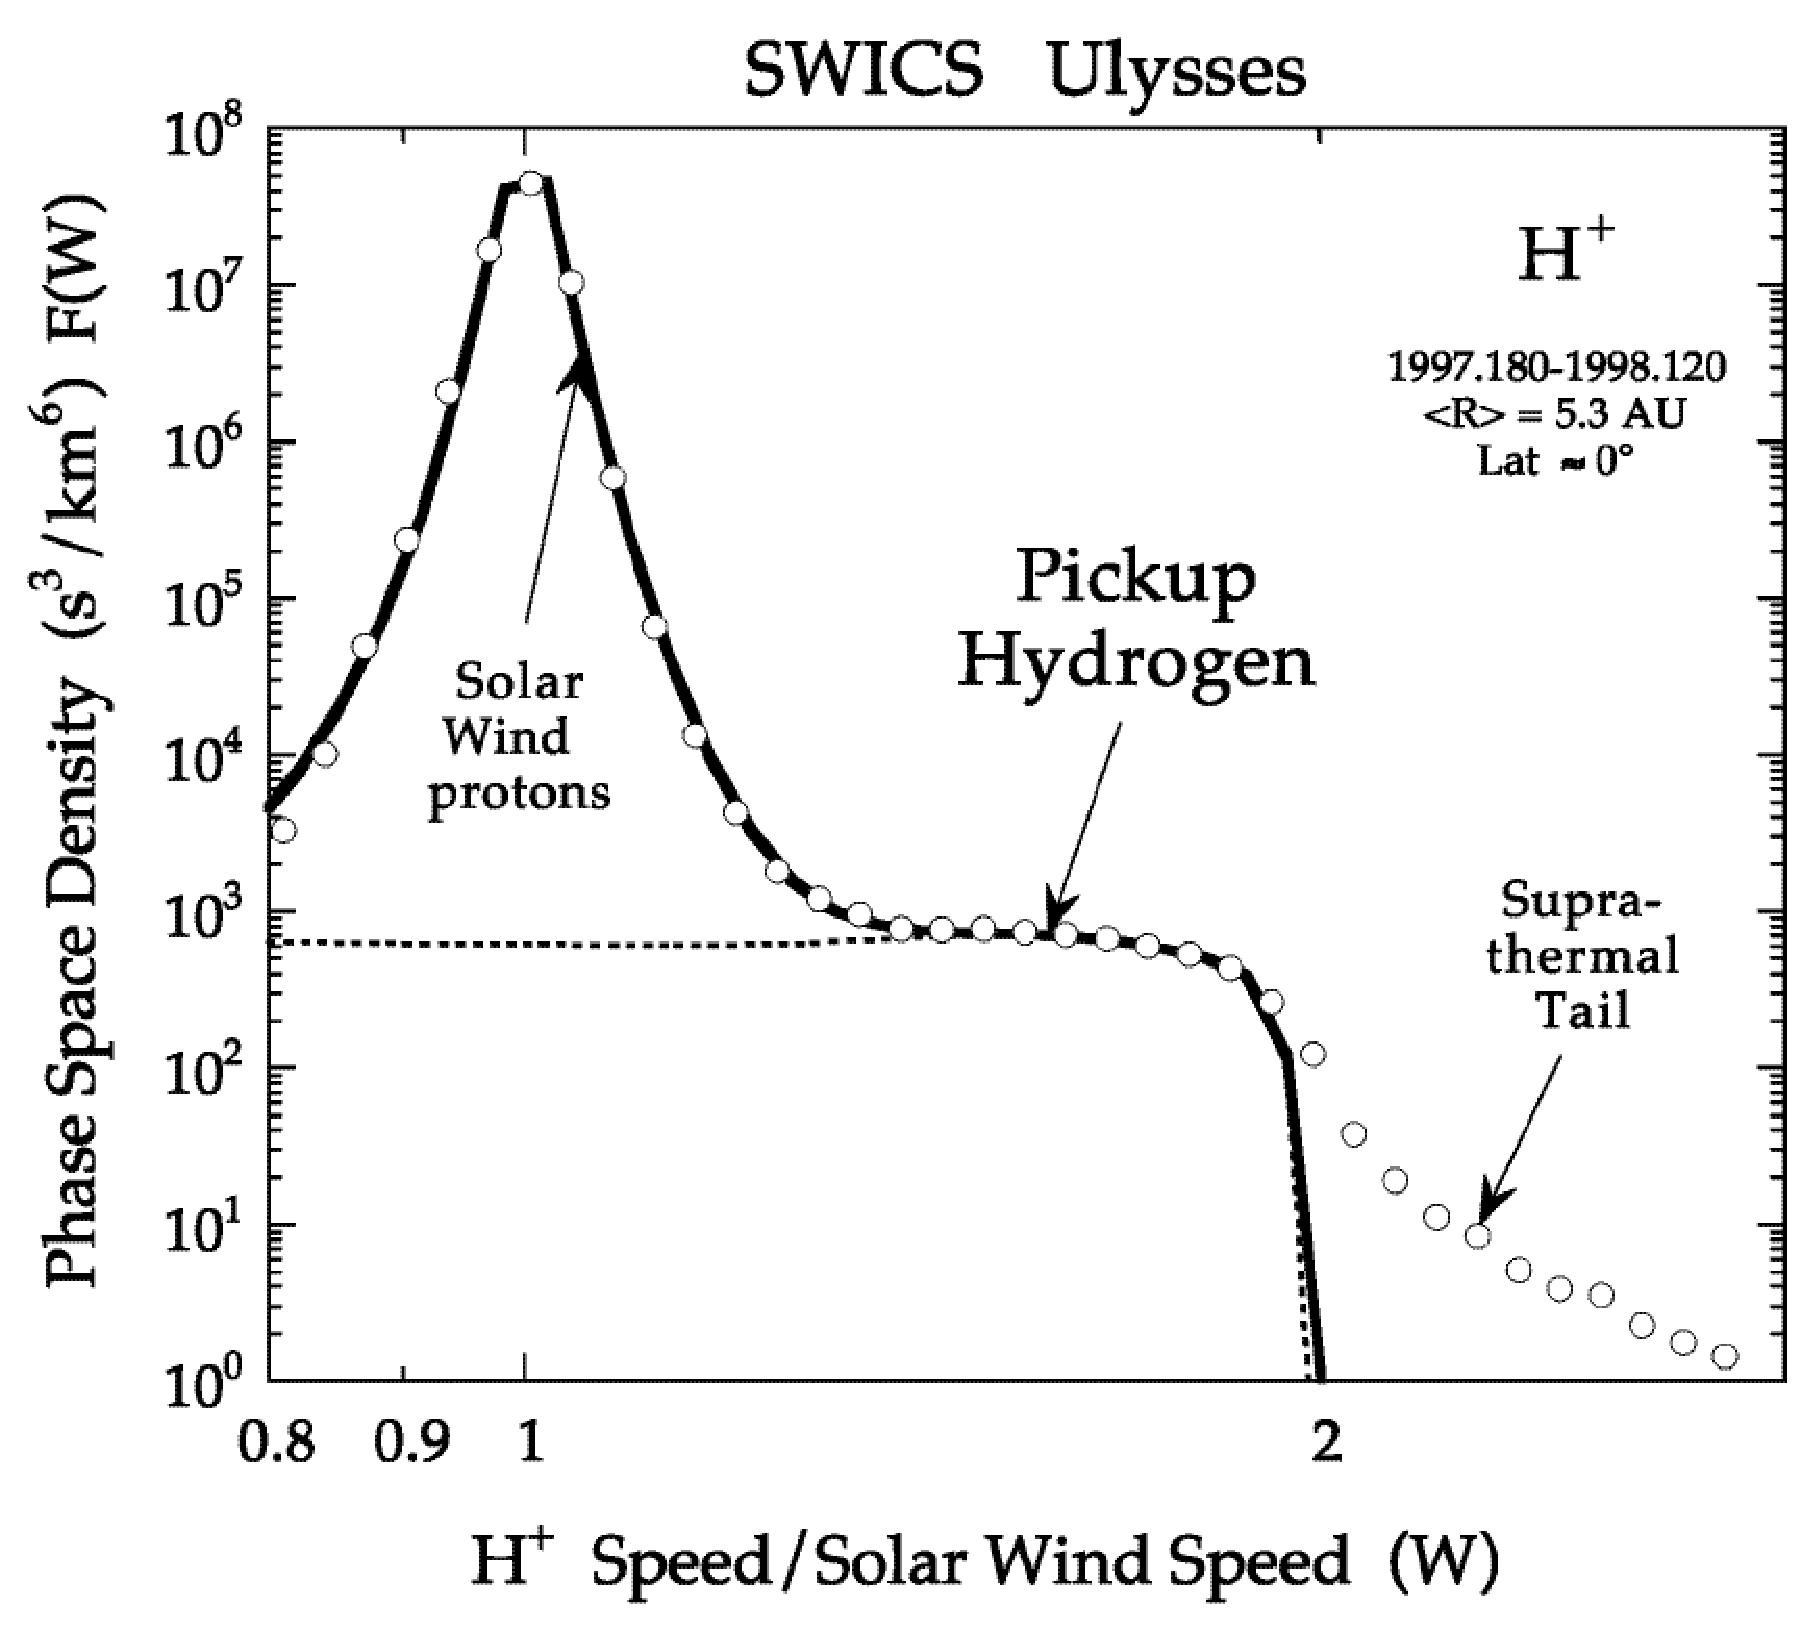
\includegraphics[width=.65\textwidth]{Chap2/H_Distribution}
%  \caption[Example of proton distributions for the quiet solar wind near 5 AU.]{Example of proton distributions for the quiet solar wind near 5 AU. Shown are the bulk distribution of the solar wind, the interstellar pickup ions that drop off at twice the solar wind speed, and the high-energy protons that make up the suprathermal tail. Figure from \citet{gloeckler01b}.}
%  \label{fig:H_Distribution}
%\end{figure}

\section{The Solar Wind}
\label{Solar Wind}

\subsection{Current Knowledge}
\label{SW Current Knowledge}
While he was not the first to postulate its existence, the physics of the solar wind was first explained by Eugene Parker in 1958 \citep{parker58}. Beginning with subsonic speeds close to the Sun, plasma accelerates away from the solar surface and reaches supersonic speeds in the corona. It continues to expand in a radial direction outward until it interacts with the material in interstellar space at the edge of the heliosphere, the Sun's sphere of influence. The wind draws the solar magnetic field along with it, creating spiral-shaped field lines as the Sun rotates \citep{parker59}. Mankind's understanding of the processes that govern the solar wind has increased as spacecraft have taken in situ measurements, but there are still some properties that remain unexplained, such as the precise origin of certain types of wind, as discussed below.

The solar wind travels a distance of one \ac{AU} before reaching Earth's orbit, where most of the current measurements have been taken (Table~\ref{tab:solar wind}). It is generally divided into two components, commonly referred to as the ``fast'' and ``slow'' solar wind. Originally, these terms were used to differentiate the wind by the speed with which it traveled, but more recent studies have shown that the two types of wind are more efficiently distinguished by their charge state composition (e.g., O$^{7+}$/O$^{6+}$) since the plasma can change speeds as it flows through space \citep{geiss95b, gloeckler03a}. Rather than the terms ``fast'' and ``slow'', more appropriate labels are descriptive of the wind's origin: ``coronal hole'' and ``streamer'' wind. These two types of wind are generated by different processes and have different compositions, temperatures, speeds, and origins.
\begin{table}[htbp]
	\centering
		\begin{tabular}{l|c|c}
		                                                               & Coronal Hole Wind & Streamer Wind     \\ \hline
      bulk speed \footnotesize{$\left(\text{km s}^{-1}\right)$}    & 750               & 400               \\ \hline
      thermal speed \footnotesize{$\left(\text{km s}^{-1}\right)$} & 32                & 35                \\ \hline
      H$^+$ density \footnotesize{$\left(\text{cm}^{-3}\right)$}   & 2.5               & 8.7               \\ \hline
      frozen-in temperature \footnotesize{$\left(\text{K}\right)$} & 8 x 10$^5$        & 1.4--1.6 x 10$^6$ \\ \hline

		\end{tabular}
	\caption[Average characteristics of the solar wind at 1 AU.]{Average characteristics of the solar wind at 1 AU. The temperature is derived from the freeze-in temperature of C$^{6+}$/C$^{5+}$, which freezes in near the solar wind source altitude. Data compiled from \citet{vonsteiger95, gloeckler98a, ipavich98, mccomas00, feldman05}.}
	\label{tab:solar wind}
\end{table}

As solar wind ions escape from the photosphere and travel up through the corona, they experience collisions with energetic electrons that ionize them to different degrees. As they travel farther through the corona, continuously accelerating, the density of coronal electrons decreases and the particles experience fewer collisions. When the timescale for ionization or recombination becomes longer than the timescale of the solar wind to expand through a density scale height, the charge state of the ion is said to be ``frozen in,'' branding the ion with the coronal region and electron temperature of its origin \citep{hundhausen68}. The streamer wind has a distinct characteristic of being enriched in elements with a low ($\le$ 10 eV) \ac{FIP} by a factor of 3--4 over the photospheric value. The coronal hole wind does not show this density enhancement, and measurements have revealed abundances of low-\ac{FIP} elements that match ratios in the photosphere \citep{vonsteiger93}. The streamer wind also has a higher and more variable freeze-in temperature than the coronal hole wind. One explanation for this describes solar plasma trapped and heated in large coronal loops that are eventually opened by interchange reconnection, releasing the plasma \citep{gosling95, fisk98, fisk99a}.

The coronal hole wind originates in the open flux regions of the Sun, which contain low-density plasma and concentrations of magnetic flux that are all the same polarity. During solar minimum these regions are clustered around the poles of the Sun, while during solar maximum they appear at all latitudes. Plasma in open flux regions is also released from flux loops, but the high concentration of open flux increases the probability that the loops will open before they can heat and fractionate the plasma. The anti-correlation between freeze-in temperature and solar wind speed shown in Table~\ref{tab:solar wind} can be interpreted in a simplistic way as a sign of different sized loops. The long-lived loops that produce the streamer wind will expand and rise slowly into the corona, where the temperatures are hotter, before being opened \citep{fisk98, fisk01a}. The short-lived loops that yield the coronal hole wind are opened while they are still small and close to the cooler surface \citep{fisk99a, fisk03, wimmer03b}.


\startappendices
 \appendix{Two-Dimensional Crank-Nicolson Scheme for a Uniform Spherical Grid}
 \label{app:CN Scheme}
 This is an example appendix.
For the diffusion process, The equation was solved using a two-dimensional implicit Crank-Nicolson scheme, which is unconditionally stable and second-order accurate in both time and space \citep{crank47}. In the conventional notation, the two-dimensional numerical scheme using central differencing can be written for a uniform Cartesian grid as 
\begin{eqnarray}
\nonumber\left(1+2\mu\right)u^{t+1}_{i,j}-\frac{\mu}{2}\left(u^{t+1}_{i+1,j}+u^{t+1}_{i-1,j}+u^{t+1}_{i,j+1}+u^{t+1}_{i,j-1}\right)\\
=\left(1-2\mu\right)u^{t}_{i,j}+\frac{\mu}{2}\left(u^{t}_{i+1,j}+u^{t}_{i-1,j}+u^{t}_{i,j+1}+u^{t}_{i,j-1}\right),
\end{eqnarray}

\noindent where $u^{t}_{i,j}$ is the value of the parameter undergoing the diffusion ($B_{r}$ in this case) at position $(i, j)$ at time \textit{t}. The von Neumann number on a uniform grid is $\mu=\xi{\Delta}t/\left({\Delta}x\right)^{2}$, where the size of the grid square is $\Delta x$ on each side, and the diffusion coefficient $\xi$ describes the speed at which the mathematical diffusion takes place. When deriving the two-dimensional Crank-Nicolson scheme in spherical coordinates, the von Neumann number is written as $\mu=\xi{\Delta}t/\left(r\Delta\theta\right)^{2}$, where $\Delta\theta=\Delta\phi$, and the cosine is replaced by the central difference of the sine to remain consistent with the discrete nature of the other terms. Care must be taken at the poles, where the central differencing is replaced by forward or backward differencing. To keep second-order accuracy with forward or backward differencing, the series must be carried out to higher-order terms in the derivation. The two-dimensional numerical scheme using central differencing can be written for a uniform spherical grid as
\begin{multline}
\left(1+\mu+\frac{\mu}{\sin^{2}\theta_{i,j}}\right)u^{t+1}_{i,j}-\frac{\mu}{2}\left[1+\frac{\left(\sin\theta_{i+1,j}-\sin\theta_{i-1,j}\right)}{4\sin\theta_{i,j}}\right]u^{t+1}_{i+1,j}\\
 -\frac{\mu}{2}\left[1-\frac{\left(\sin\theta_{i+1,j}-\sin\theta_{i-1,j}\right)}{4\sin\theta_{i,j}}\right]u^{t+1}_{i-1,j}-\frac{\mu}{2}\frac{1}{\sin^{2}\theta_{i,j}}u^{t+1}_{i,j+1}-\frac{\mu}{2}\frac{1}{\sin^{2}\theta_{i,j}}u^{t+1}_{i,j-1}\\
 =\left(1-\mu-\frac{\mu}{\sin^{2}\theta_{i,j}}\right)u^{t+1}_{i,j}+\frac{\mu}{2}\left[1+\frac{\left(\sin\theta_{i+1,j}-\sin\theta_{i-1,j}\right)}{4\sin\theta_{i,j}}\right]u^{t+1}_{i+1,j}\\
 +\frac{\mu}{2}\left[1-\frac{\left(\sin\theta_{i+1,j}-\sin\theta_{i-1,j}\right)}{4\sin\theta_{i,j}}\right]u^{t+1}_{i-1,j}+\frac{\mu}{2}\frac{1}{\sin^{2}\theta_{i,j}}u^{t+1}_{i,j+1}+\frac{\mu}{2}\frac{1}{\sin^{2}\theta_{i,j}}u^{t+1}_{i,j-1}.
 \label{CN Spherical}
\end{multline}

%Although it is unconditionally stable, a marching scheme such as this will depend on the value of $\mu$ for its accuracy. A lower choice of $\mu$ will lead to a more accurate solution at the expense of computational resources (i.e., a smaller time step ${\Delta}t$), while a higher value of $\mu$ will arrive at a solution more rapidly but with less accuracy (a larger time step). In this model, the value of the coefficient $\xi$ describes the speed of the mathematical relaxation and, since it does not describe a physical process, can be chosen arbitrarily. Thus the only restriction for this scheme will lie in keeping $\mu$ small for accuracy and assigning either $\xi$ or ${\Delta}t$. It can be seen that when $\mu$ is held constant, any choice for either $\xi$ or ${\Delta}t$ will lead to the same solution. A value of $\mu=1/4$ was chosen, with an arbitrary time step of ${\Delta}t=0.1$ s, and studied several different grid resolutions, with a grid size of 2.5$^\circ$ x 2.5$^\circ$ (72 x 144 grid spaces) on a uniform spherical grid used for the comparisons in this paper. The relaxation was allowed to continue on a sphere of $r=R_{\sun}$ until the difference in magnetic field magnitude between any cell and its neighbor was of order $10^{-1}{\mu}T$.

 
\startbibliography
 \begin{singlespace} % Bibliography must be single spaced
  \bibliography{References}   % Use the BibTeX file ``References.bib''.
 \end{singlespace}

% An external Abstract that can be printed at the end of the document, 
% for separate submission to Rackham. Comment it out when not needed. - jg
%\startextabstractpage
%{The Title of Your Dissertation}{Your Name}{Chair: Albert Einstein}
%Emerging storage technologies offer an alternative to disk that is durable and allows faster data access.
Flash memory, made popular by mobile devices, provides block access with low latency random reads.
New nonvolatile memories (NVRAM) are expected in upcoming years, presenting DRAM-like performance alongside persistent storage.
Wheres both technologies accelerate data accesses due to increased raw speed, used merely as disk replacements they may fail to achieve their full potentials.
Flash's asymmetric read/write access (i.e., reads execute faster than writes) opens new opportunities to optimize Flash-specific access.
Similarly, NVRAM's low latency persistent accesses allow new designs for high performance failure-resistant applications.

This thesis addresses software and hardware system design for such storage technologies.
First, I investigate analytics query optimization for Flash, expecting Flash's fast random access to require new query planning.
While intuition suggests scan and join selection should shift between disk and Flash, I find that query plans chosen assuming disk are already near-optimal for Flash.
Second, I examine new opportunities for durable, recoverable transaction processing with NVRAM.
Existing disk-based recovery mechanisms impose large software overheads, yet updating data in-place requires frequent device synchronization that limits throughput.
I introduce a new design, \GroupCommit, to amortize synchronization delays over many transactions, increasing throughput at some cost to transaction latency.
Finally, I propose a new framework for persistent programming and memory systems to enable high performance recoverable data structures with NVRAM, extending memory consistency with persistent semantics to introduce \emph{memory persistency}.

%\label{ExtAbstract}

\end{document}
